\chapter{Experimental Results} 
\label{ch:results}

In this chapter we evaluate the performance of the proposed approach, described 
in \autoref{ch:evaluation}. Two experiments are performed: In the first 
experiment, we compare our approach running on three different platforms,
two of them computationally restricted. The platforms are a laptop 
computer, a UP-Board, and the onboard computer of an AscTec 
Hummingbird\footnote{
http://www.asctec.de/en/uav-uas-drones-rpas-roav/asctec-hummingbird/}.
Additionally, we also run the default implementation of VINS-Mono on the 
laptop. This first experiment was performed on all sequences of the EuRoC 
dataset \citep{Burri2016EuRoC}. In the second experiment our approach is 
deployed on a AscTec Neo\footnote{
http://www.asctec.de/en/uav-uas-drones-rpas-roav/asctec-neo/}, a real \ac{UAV}.

\section{Experimental Settings} \label{sec:results_dataset}

\subsection{First Experiment}\label{subsec:firstexperiment}

\subsubsection{Hardware Platforms} \label{subsubsec:hardwareplatforms1}
The tests are performed on a Laptop with an Intel i7-6600U CPU running at up to 
3.4 GHz, on a UP Board with an Intel Atom x5-Z8350 CPU running at up to 1.92 
GHz, and on the onboard computer of an AscTec Hummingbird with an Intel Atom 
E3845 CPU running at 1.92GHz.

\subsubsection{Metrics}\label{subsubsec:metrics}
We measure the same two metrics (accuracy and per-frame optimization time) 
as described in the evaluation \autoref{sec:metrics}. However, the metrics 
are measured over all the sequences combined. In addition for each individual 
sequence, the whole trajectory is aligned to the ground truth using a 
\textit{sim3} trajectory alignment according to the method proposed in 
\citep{Umeyama1991}. Then the RMSE position error over the aligned trajectory is 
calculated. We also highlight the maximal per-frame optimization time for each 
sequence to ensure that real-time performance is fulfilled.

\subsection{Second Experiment}\label{subsec:secondexperiment}
\subsubsection{Hardware Platforms} \label{subsubsec:hardwareplatforms2}

In the second experiment, the proposed pipeline has been deployed on an
 AscTec Neo, equipped with an Intel NUC which has much more computational power 
than required. Due to time limits the pipeline could not be deployed on 
a \ac{UAV} with a more restricted onboard computer. However the results in 
\autoref{subsec:result1} show that a 
similar accuracy on a less powerful platform can be assumed. \\

The \ac{VIO} pose estimation uses camera and \ac{IMU} measurements obtained 
by the VI-Sensor described in \citep{nikolic2014synchronized}. Instead of the 
front-looking camera an additional down-looking camera has been used. The 
calibration between the additional camera and the \ac{IMU} was performed using 
the \textit{kalibr} toolbox \cite{furgale2013kalibr} from 
\ac{ASL}\footnote{ https://github.com/ethz-asl/kalibr}. In 
addition, the proposed \ac{VIO} pose estimation has been fused with the onboard 
\ac{IMU} of the \ac{UAV} using an \ac{EKF} \ac{MSF} framework from 
\ac{ASL}\footnote{ https://github.com/ethz-asl/ethzasl\_msf} described in 
\citep{lynen2013robust}. \textit{kalibr} toolbox was 
again used for the calibration between the onboard \ac{IMU} and the camera 
frame. \\

\section{Experiments}\label{sec:experiments}
Both experiments are evaluated with the parameters of our approach set to 
the following:
\begin{itemize}
  \item $n_{\text{features\_tracked}} = 120$ features.
  \item $n_{\text{oldest\_keyframes}} = 4$ keyframes.
  \item $n_{\text{observed\_keyframes}} = 6$ (key-)frames. 
\end{itemize}


\subsection{First Experiment}\label{subsec:experiment1}
We evaluate our proposed approach using the EuRoC micro aerial vehicle dataset 
\citep{Burri2016EuRoC}. This dataset provides stereo WVGA monochrome images at 
20Hz and temporally synchronized \ac{IMU} measurements at 200Hz from a 
micro-aerial vehicle manually piloted around three different indoor 
environments. Within each environment three qualitative difficulties are 
provided. For example, Machine Hall 01 is ``easy'' containing 
rather slow motions, while Machine Hall 05 is much more challenging, 
introducing fast motions, poor illuminations, etc. Each sequence 
provides a ground truth trajectory given by a Leica MS50 laser tracker for the 
Machine Hall environment and by a Vicon motion capture system for the 
other two environments. Only the images from the left camera are used for the 
evaluation.

All sequences of the dataset are used to show the performance of 
our approach in as many different scenarios as possible. 
As comparison the default VINS-Mono implementation running on the Laptop is 
also evaluated.

\subsection{Second Experiment}\label{subsec:experiment2}

Due to time limits the test were limited to hover at the current position. The 
pose estimations of the \ac{MSF} were recorded together with ground truth 
provided by a Vicon motion capture system.



\section{Results}\label{sec:results}

\subsection{First Experiment}\label{subsec:result1}

First and most important, with our approach the optimization time is below 100 
milliseconds in all sequences, compared to the default VINS-Mono running on the 
UP-Board. The results are listed in \autoref{tab:EuRoC_results_time}. We can see 
that the accuracy of our approach has decreased compared to the default version 
of VINS-Mono running on the laptop, best noticeable in the median in the box 
plot in \autoref{fig:acc_result}. Furthermore, one can see that the accuracy of 
our approach on the Laptop and the UP-Board is very similar. The only difference 
on the UP-Board is the increase in computational time, as shown in 
\autoref{fig:time_result}. This indicates the robustness of our algorithm, 
meaning the algorithm does not run at the limit on the UP Board. On the AscTec 
Hummingbird the accuracy is slightly worse. We assume the reason is the older 
CPU generation which lacks of the Intel Burst function for short-time 
overclocking of the CPU. The RMSE in \autoref{tab:EuRoC_results} shows that our 
approach even outperforms the default VINS-Mono in the ``easy'' sequences of the 
Machine Hall and V1 environment. Whereas the default VINS-Mono implementation 
running on the laptop achieves higher accuracy in the difficult sequences. 
During the fast movements of these sequences the feature tracker is not as 
accurate as during slow movements. We assume that during fast movements, more 
constraints from the observed features improve the accuracy. During slow 
movements the feature tracking is very accurate and running the \ac{BA} 
optimization with only a reduced number of feature constraints is sufficient 
enough, allowing for more iteration in the limited solving time. This results in 
a higher accuracy.
\begin{minipage}[H]{1\linewidth}
\vspace{-5pt}
\begin{figure}[H]
\centering
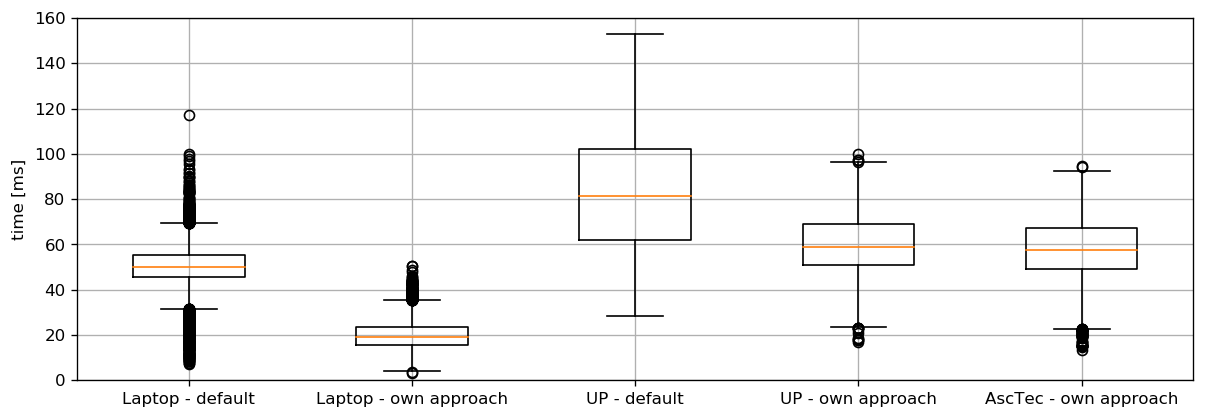
\includegraphics[width=0.96\textwidth]{images/result_time}
\caption{Boxplot summarizing the whole optimization time (optimization and 
marginalization) for the \ac{VIO} pipeline over all sequences of the EuRoC 
dataset. The default VINS-Mono implementation running on a laptop and on a UP 
Board is compared with our own approach running on a laptop, a UP-Board and on 
the onboard computer of an AscTec Hummingbird \ac{UAV}.}
\label{fig:time_result}
\end{figure}
\vspace{-15pt}
\begin{figure}[H]
\centering
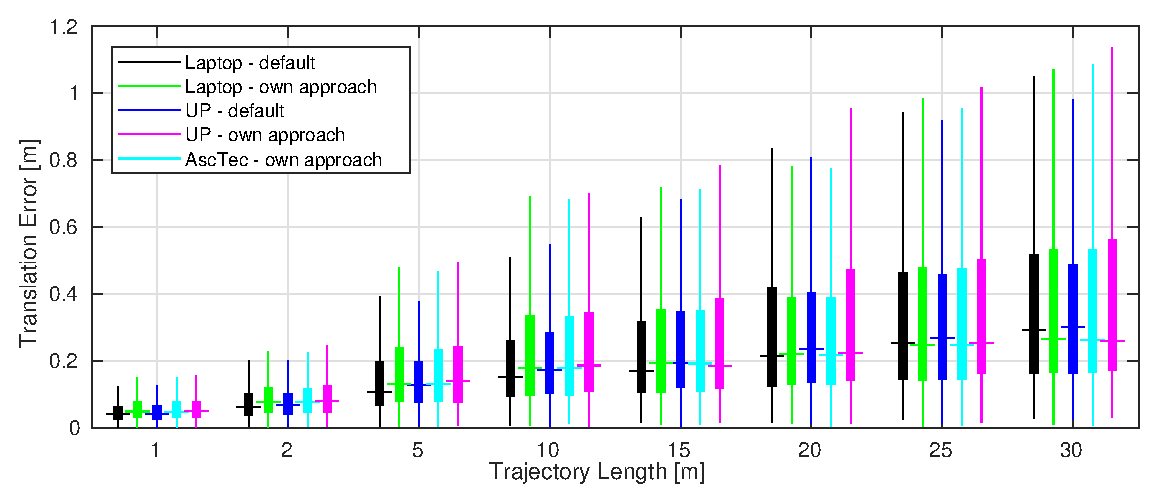
\includegraphics[width=0.96\textwidth]{images/acc_result}
\caption{Boxplot summarizing the translation error statistic for the \ac{VIO}
pipeline over all sequences of the EuRoC dataset. The default VINS-Mono 
implementation running on a laptop and on a UP Board is compared with our own 
approach running on a laptop, a UP-Board and on the onboard computer of an 
AscTec Hummingbird \ac{UAV}. Errors were computed using the metric described in 
\autoref{subsec:accuracy} for trajectory segments of length \{$1, 2, 5, 10, 15, 
20, 25, 30$\} m.}
\label{fig:acc_result}
\end{figure}
\end{minipage}


\begin{table}[H]
\centering
\begin{tabular}{l|c|c|c|c|c}
 & \begin{tabular}{@{}c@{}} Laptop \\ default \\ VINS-Mono \end{tabular} & 
 \begin{tabular}{@{}c@{}} UP Board \\ default \\ VINS-Mono \end{tabular} & 
Laptop & UP Board
 & \begin{tabular}{@{}c@{}} AscTec \\ Hummingbird \end{tabular} \\
 \hline
MH 01 - easy & 0.427 & 0.284 & 0.139 & 0.140 & 0.174 \\
MH 02 - easy & 0.238 & 0.375 & 0.179 & 0.180 & 0.149 \\
MH 03 - medium & 0.211 & 0.246 & 0.175 & 0.177 & 0.144 \\
MH 04 - difficult & 0.223 & 0.365 & 0.276 & 0.262 &  0.232 \\
MH 05 - difficult & 0.351 & 0.361 & 0.564 &  0.548 & 0.557 \\
\hline
V1 01 - easy &  0.142 & 0.116 & 0.066 & 0.066 & 0.095 \\
V1 02 - medium & 0.063 & 0.062 & 0.126& 0.110 & 0.085 \\
V1 03 - difficult & 0.091 & 0.147 & 0.126 & 0.127 & 0.110 \\
\hline
V2 01 - easy & 0.066 & 0.087 & 0.067 & 0.067 & 0.074\\
V2 02 - medium & 0.090 & 0.087 & 0.093 & 0.094 & 0.095\\
V2 03 - difficult & 0.123 & 0.187 & 0.172 & 0.172 & 0.167 \\
\end{tabular}
\caption{Absolute translation errors (RMSE) in meters for all sequences of the 
EuRoC dataset. The default VINS-Mono implementation running on a laptop is 
compared with our own approach running on a laptop, a UP-Board and on the 
onboard computer of an AscTec Hummingbird \ac{UAV}. Errors have been computed 
after the estimated trajectories were aligned with the ground truth trajectory 
using the method proposed in \citep{Umeyama1991}.}
\label{tab:EuRoC_results}
\end{table}


\begin{table}[H]
\centering
\begin{tabular}{l|c|c|c|c|c}
 & \begin{tabular}{@{}c@{}} Laptop \\ default \\ VINS-Mono \end{tabular} & 
 \begin{tabular}{@{}c@{}} UP Board \\ default \\ VINS-Mono \end{tabular} & 
Laptop & UP Board
 & \begin{tabular}{@{}c@{}} AscTec \\ Hummingbird \end{tabular} \\
 \hline
MH 01 - easy & 86.1 & 148.2 & 35.9 & 97.3 & 94.6 \\
MH 02 - easy & 99.9 & 148.8 & 40.9 & 95.9 & 94.0 \\
MH 03 - medium & 70.3 & 145.8 & 41.2 & 99.7 & 89.6 \\
MH 04 - difficult & 97.9 & 137.4 & 47.7 & 96.0 & 91.0 \\
MH 05 - difficult & 80.6 & 135.2 & 46.2 &  88.6 & 89.6 \\
\hline
V1 01 - easy &  117.2 & 152.9 & 45.4 & 95.5 & 91.5\\
V1 02 - medium & 65.9 & 125.6 & 42.8 & 95.6 & 80.8 \\
V1 03 - difficult & 66.7 & 135.7 & 44.2 & 87.6 & 88.5 \\
\hline
V2 01 - easy & 71.2 & 135.5 & 38.9 & 88.9 & 91.6\\
V2 02 - medium & 66.7 & 118.8 & 39.7 & 97.4 & 87.6 \\
V2 03 - difficult & 65.1 & 129.5 & 50.7 & 87.1 & 80.4 \\
\end{tabular}
\caption{Maximal optimization time in milliseconds for all sequences of the 
EuRoC dataset. The default VINS-Mono implementation running on a laptop is 
compared with our own approach running on a laptop, a UP-Board and on the 
onboard computer of an AscTec Hummingbird \ac{UAV}.}
\label{tab:EuRoC_results_time}
\end{table}


\subsection{Second Experiment}\label{subsec:result2}
Since the \ac{UAV} is supposed to hover, the relative pose should stay at zero 
for $x, y,$ and $z$. We can see that in all axis, there exist a 
noticeable error in the state estimate of the \ac{MSF} filter, shown in 
\autoref{fig:res_x}, \autoref{fig:res_y}, and \autoref{fig:res_z}. We assume 
that the main reason for this behavior is that the filter parameters were not 
optimized. The test was performed with default filter values and due to time 
restrictions, no parameter tuning for VINS-Mono and/or our approach could be 
done. The calibration between the down-looking camera and the on-board \ac{IMU} 
has also some potential for improvement. 

\begin{figure}[H]
\centering
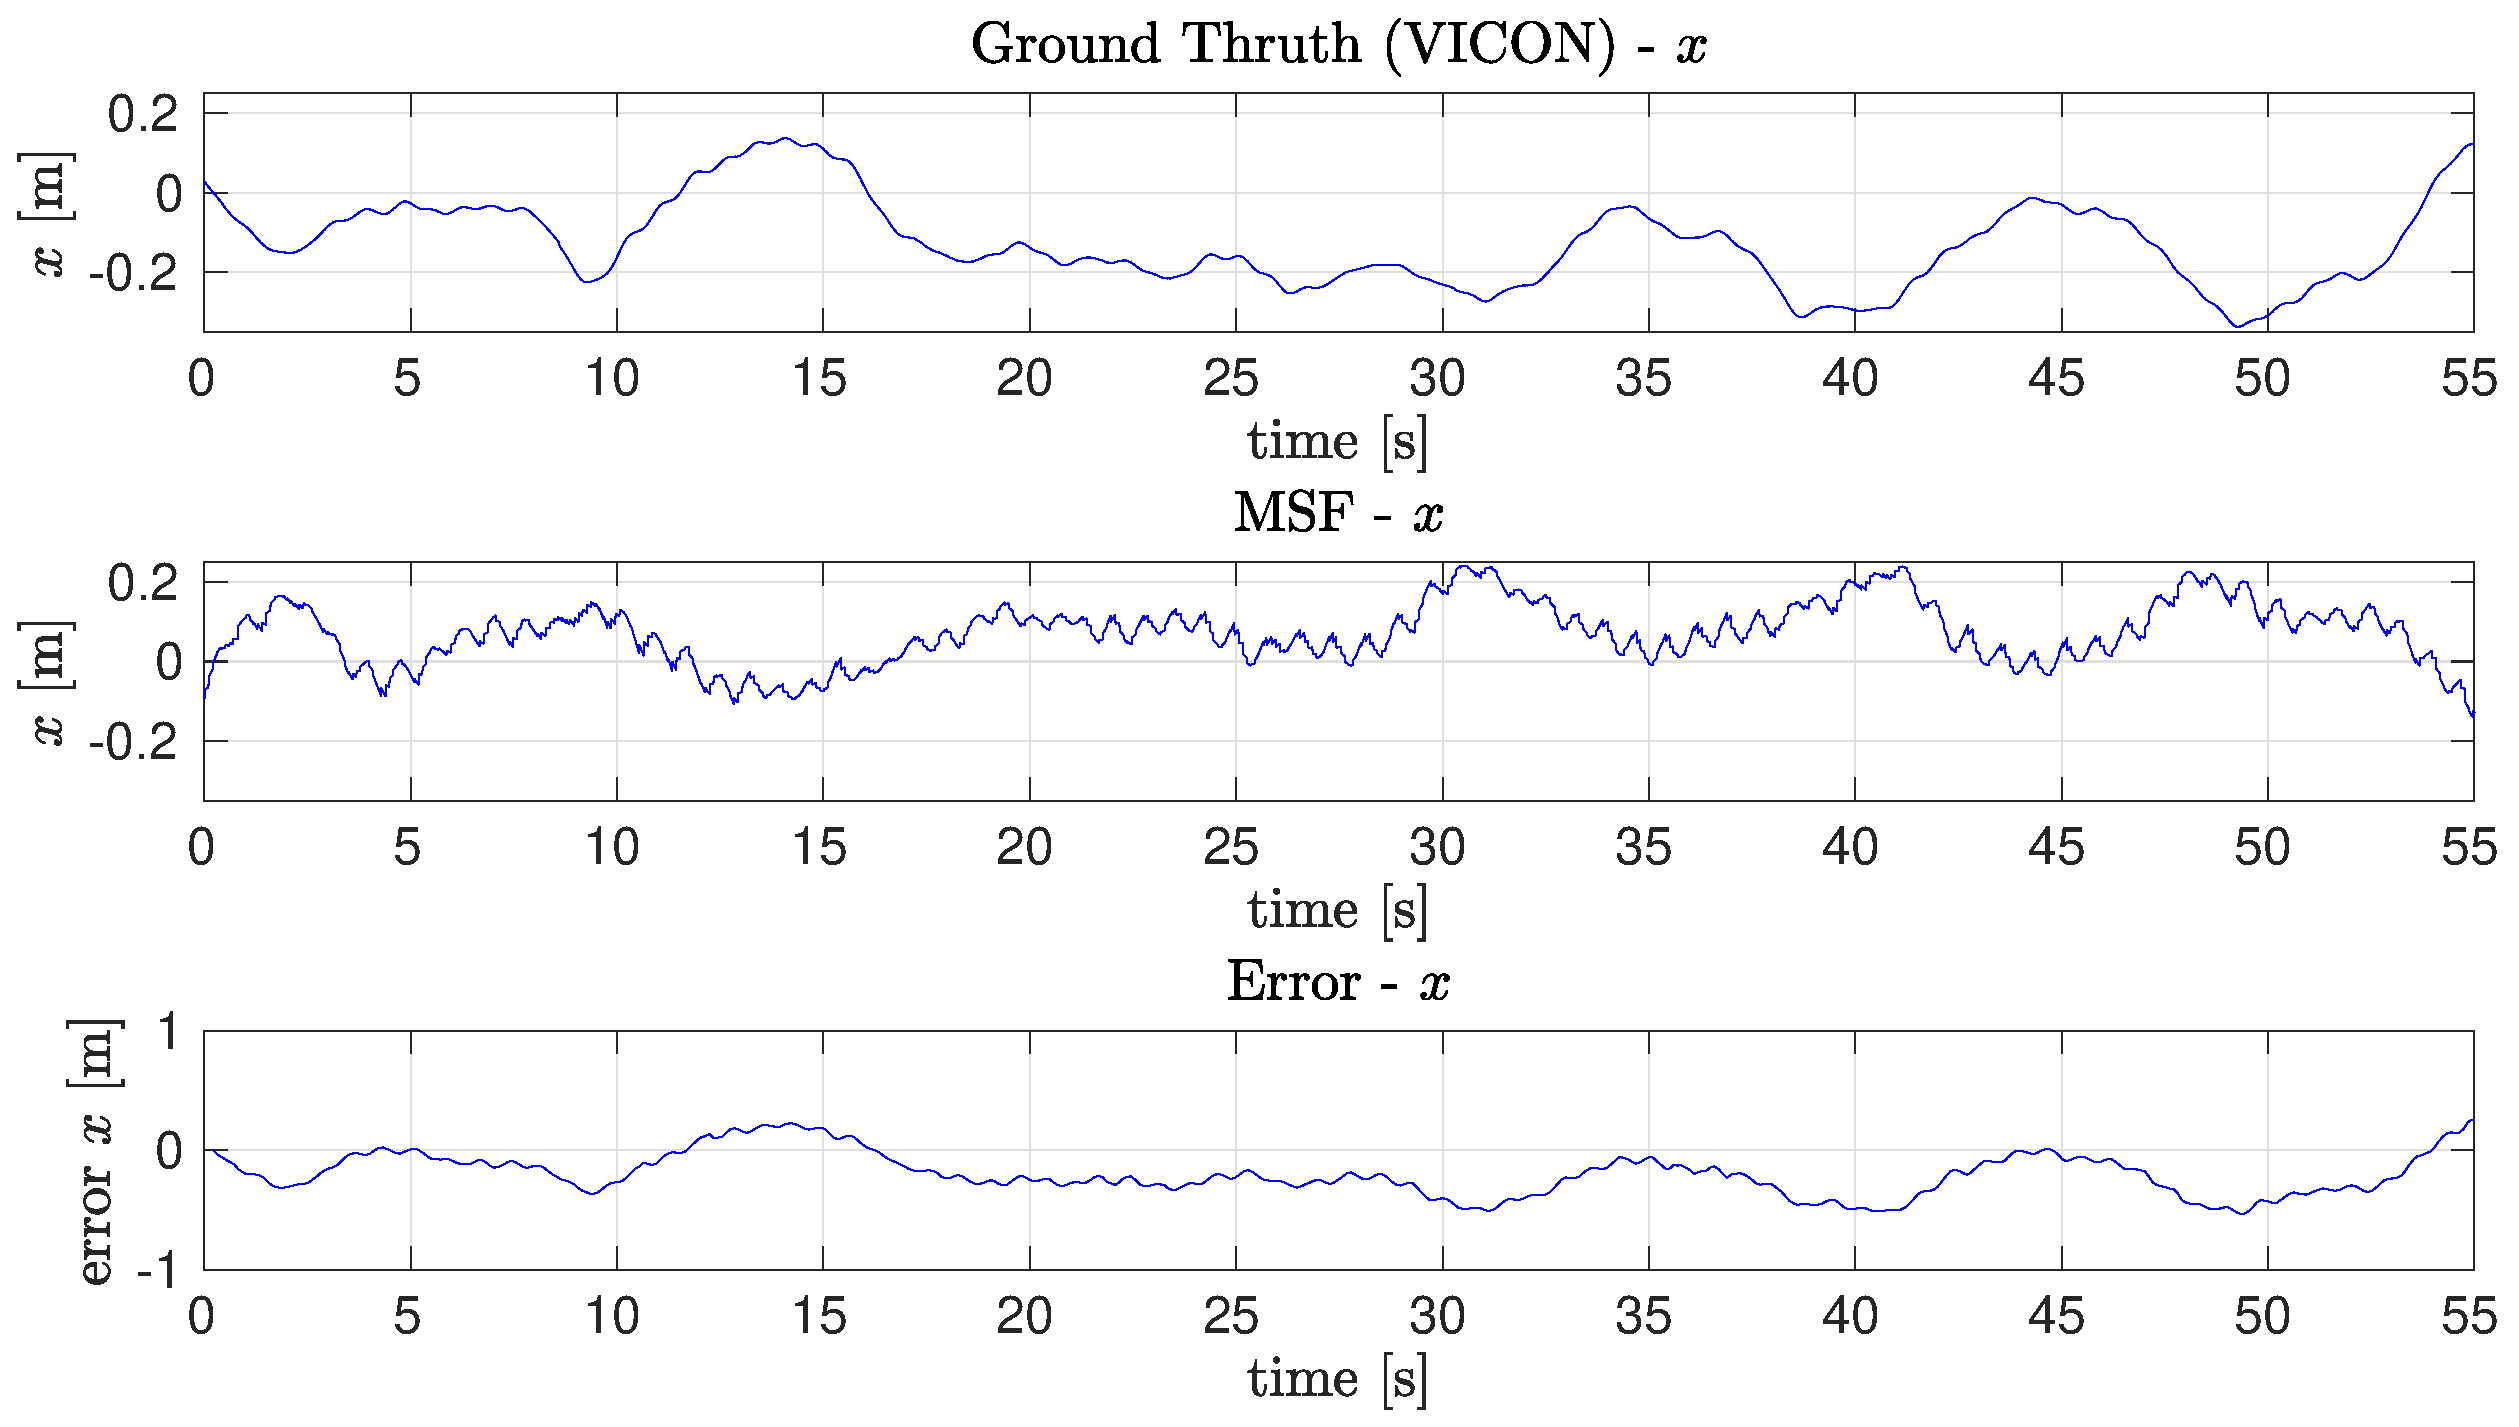
\includegraphics[width=1\textwidth]{images/res_x}
\caption{Relative pose estimation, while the \ac{UAV} is hovering, in the $x$ 
axis of the \ac{MSF} filter and the Vicon ground truth, and the difference 
between them.}
\label{fig:res_x}
\end{figure}

\begin{figure}[H]
\centering
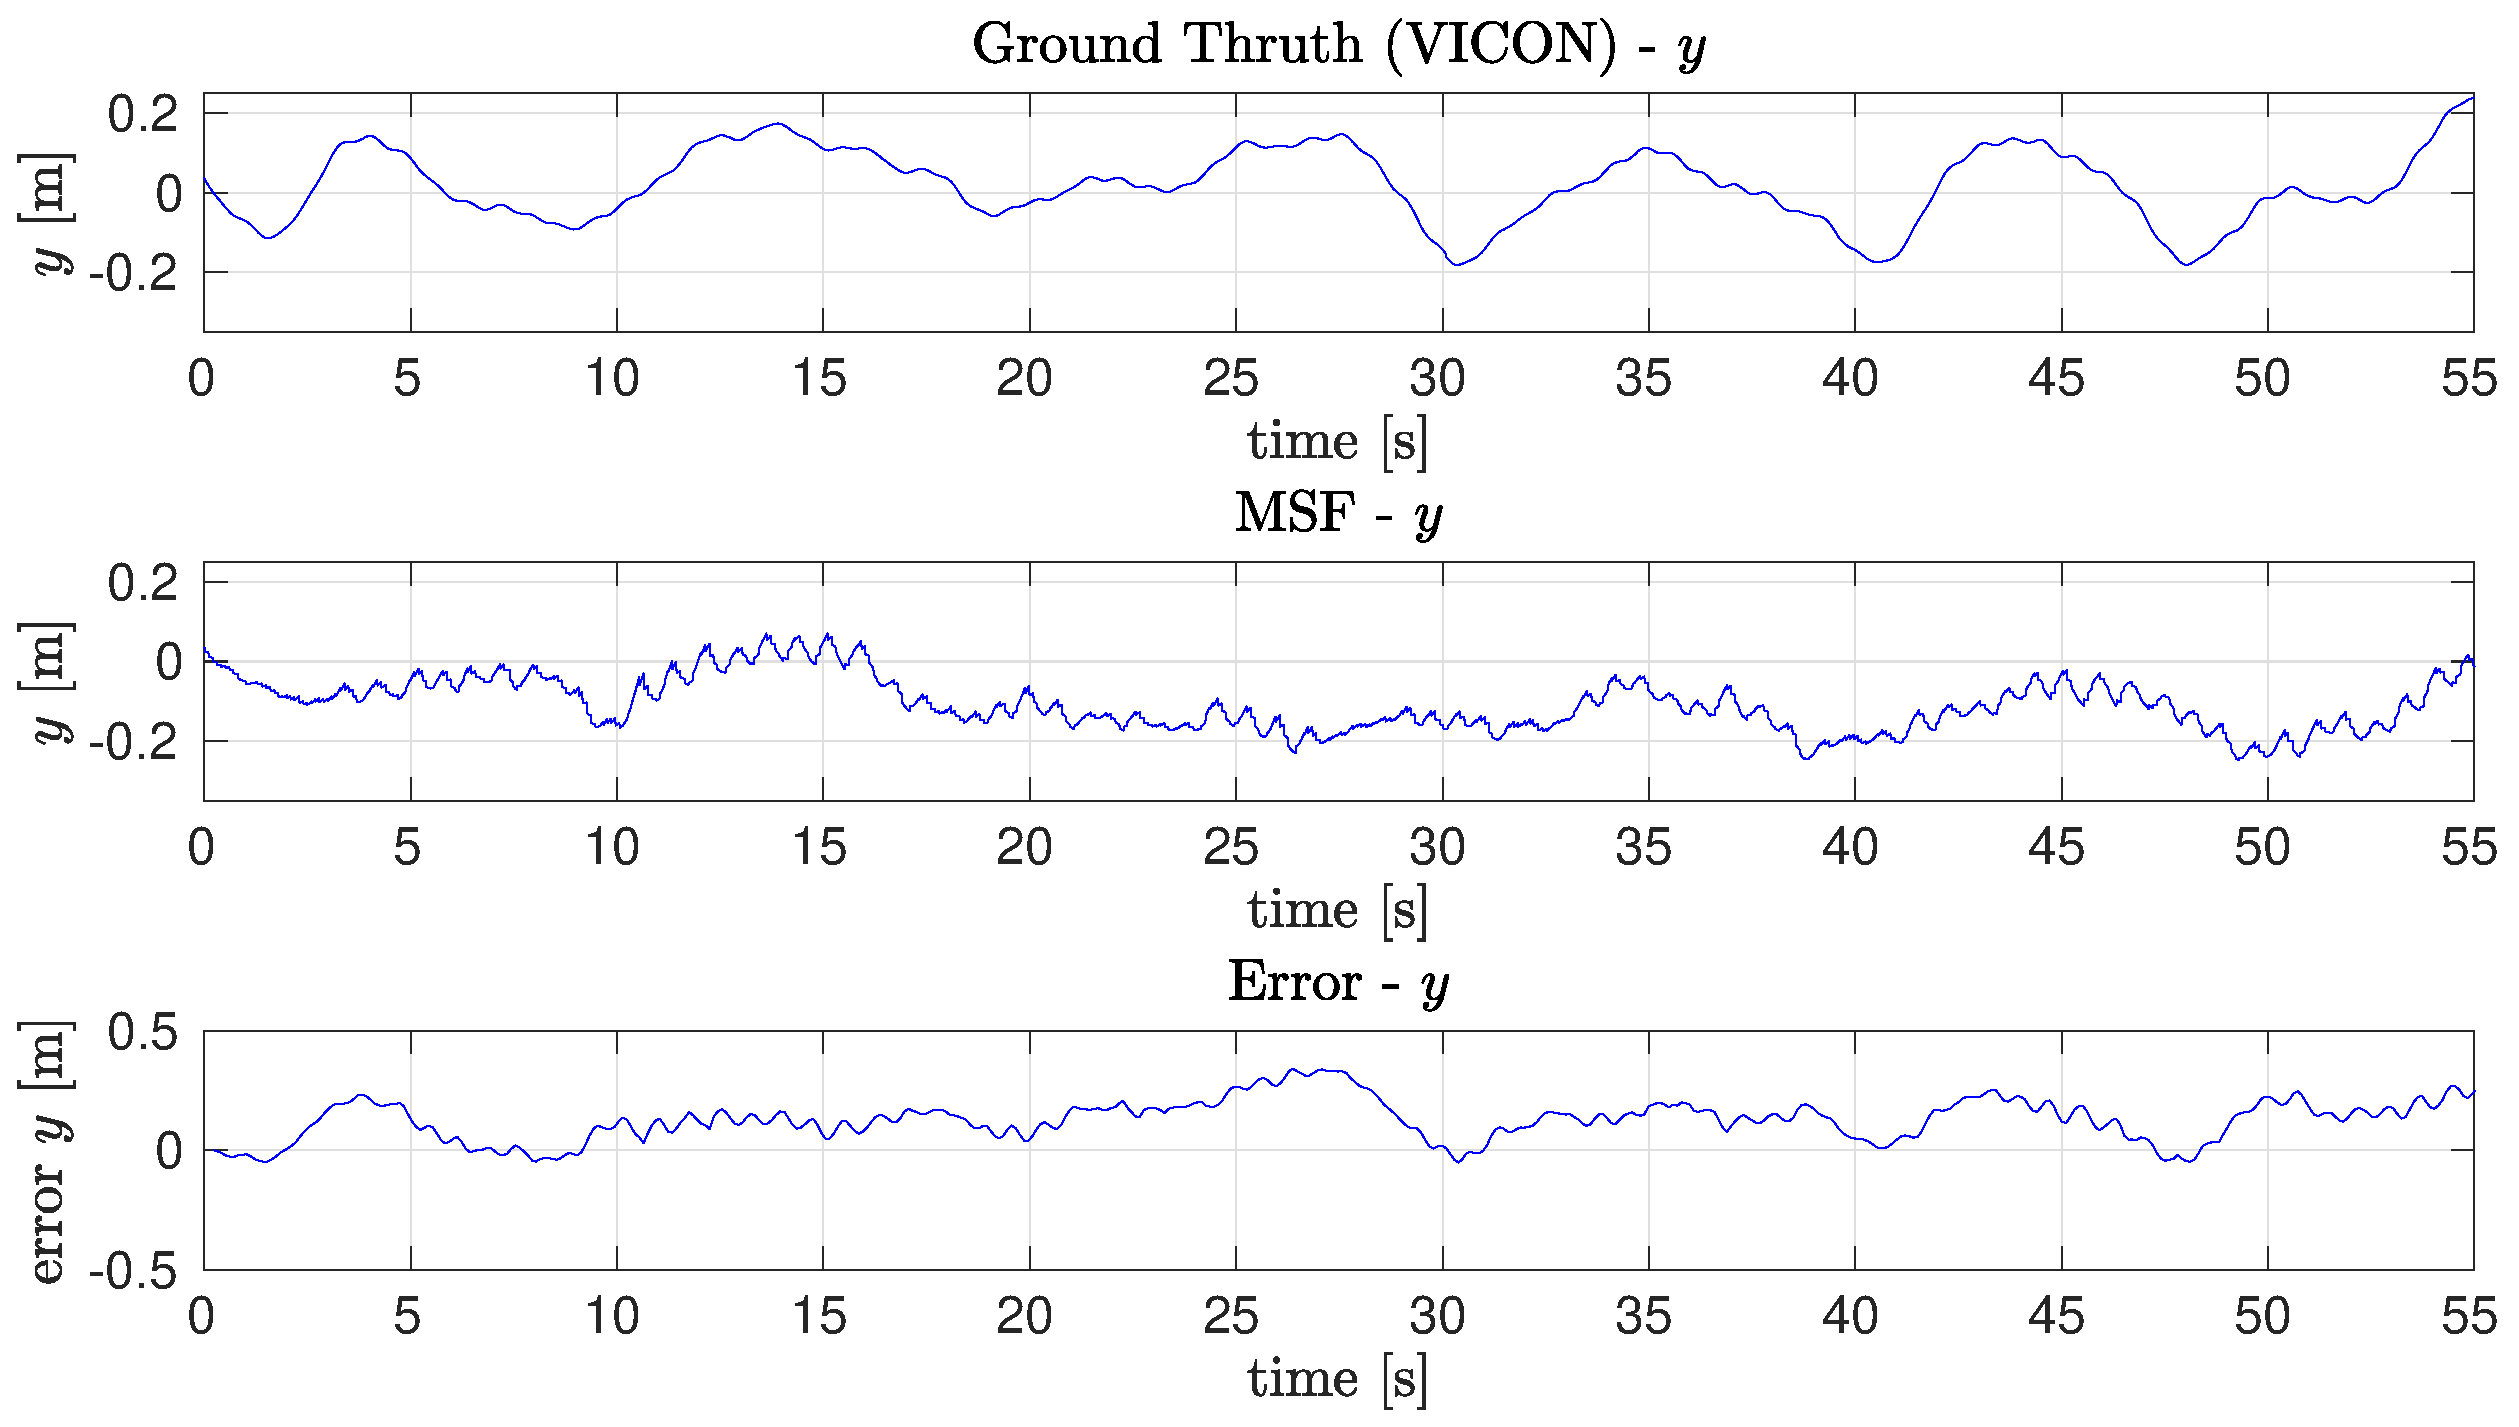
\includegraphics[width=1\textwidth]{images/res_y}
\caption{Relative pose estimation, while the \ac{UAV} is hovering, in the $y$ 
axis of the \ac{MSF} filter and the Vicon ground truth, and the difference 
between them.}
\label{fig:res_y}
\end{figure}

\begin{figure}[H]
\centering
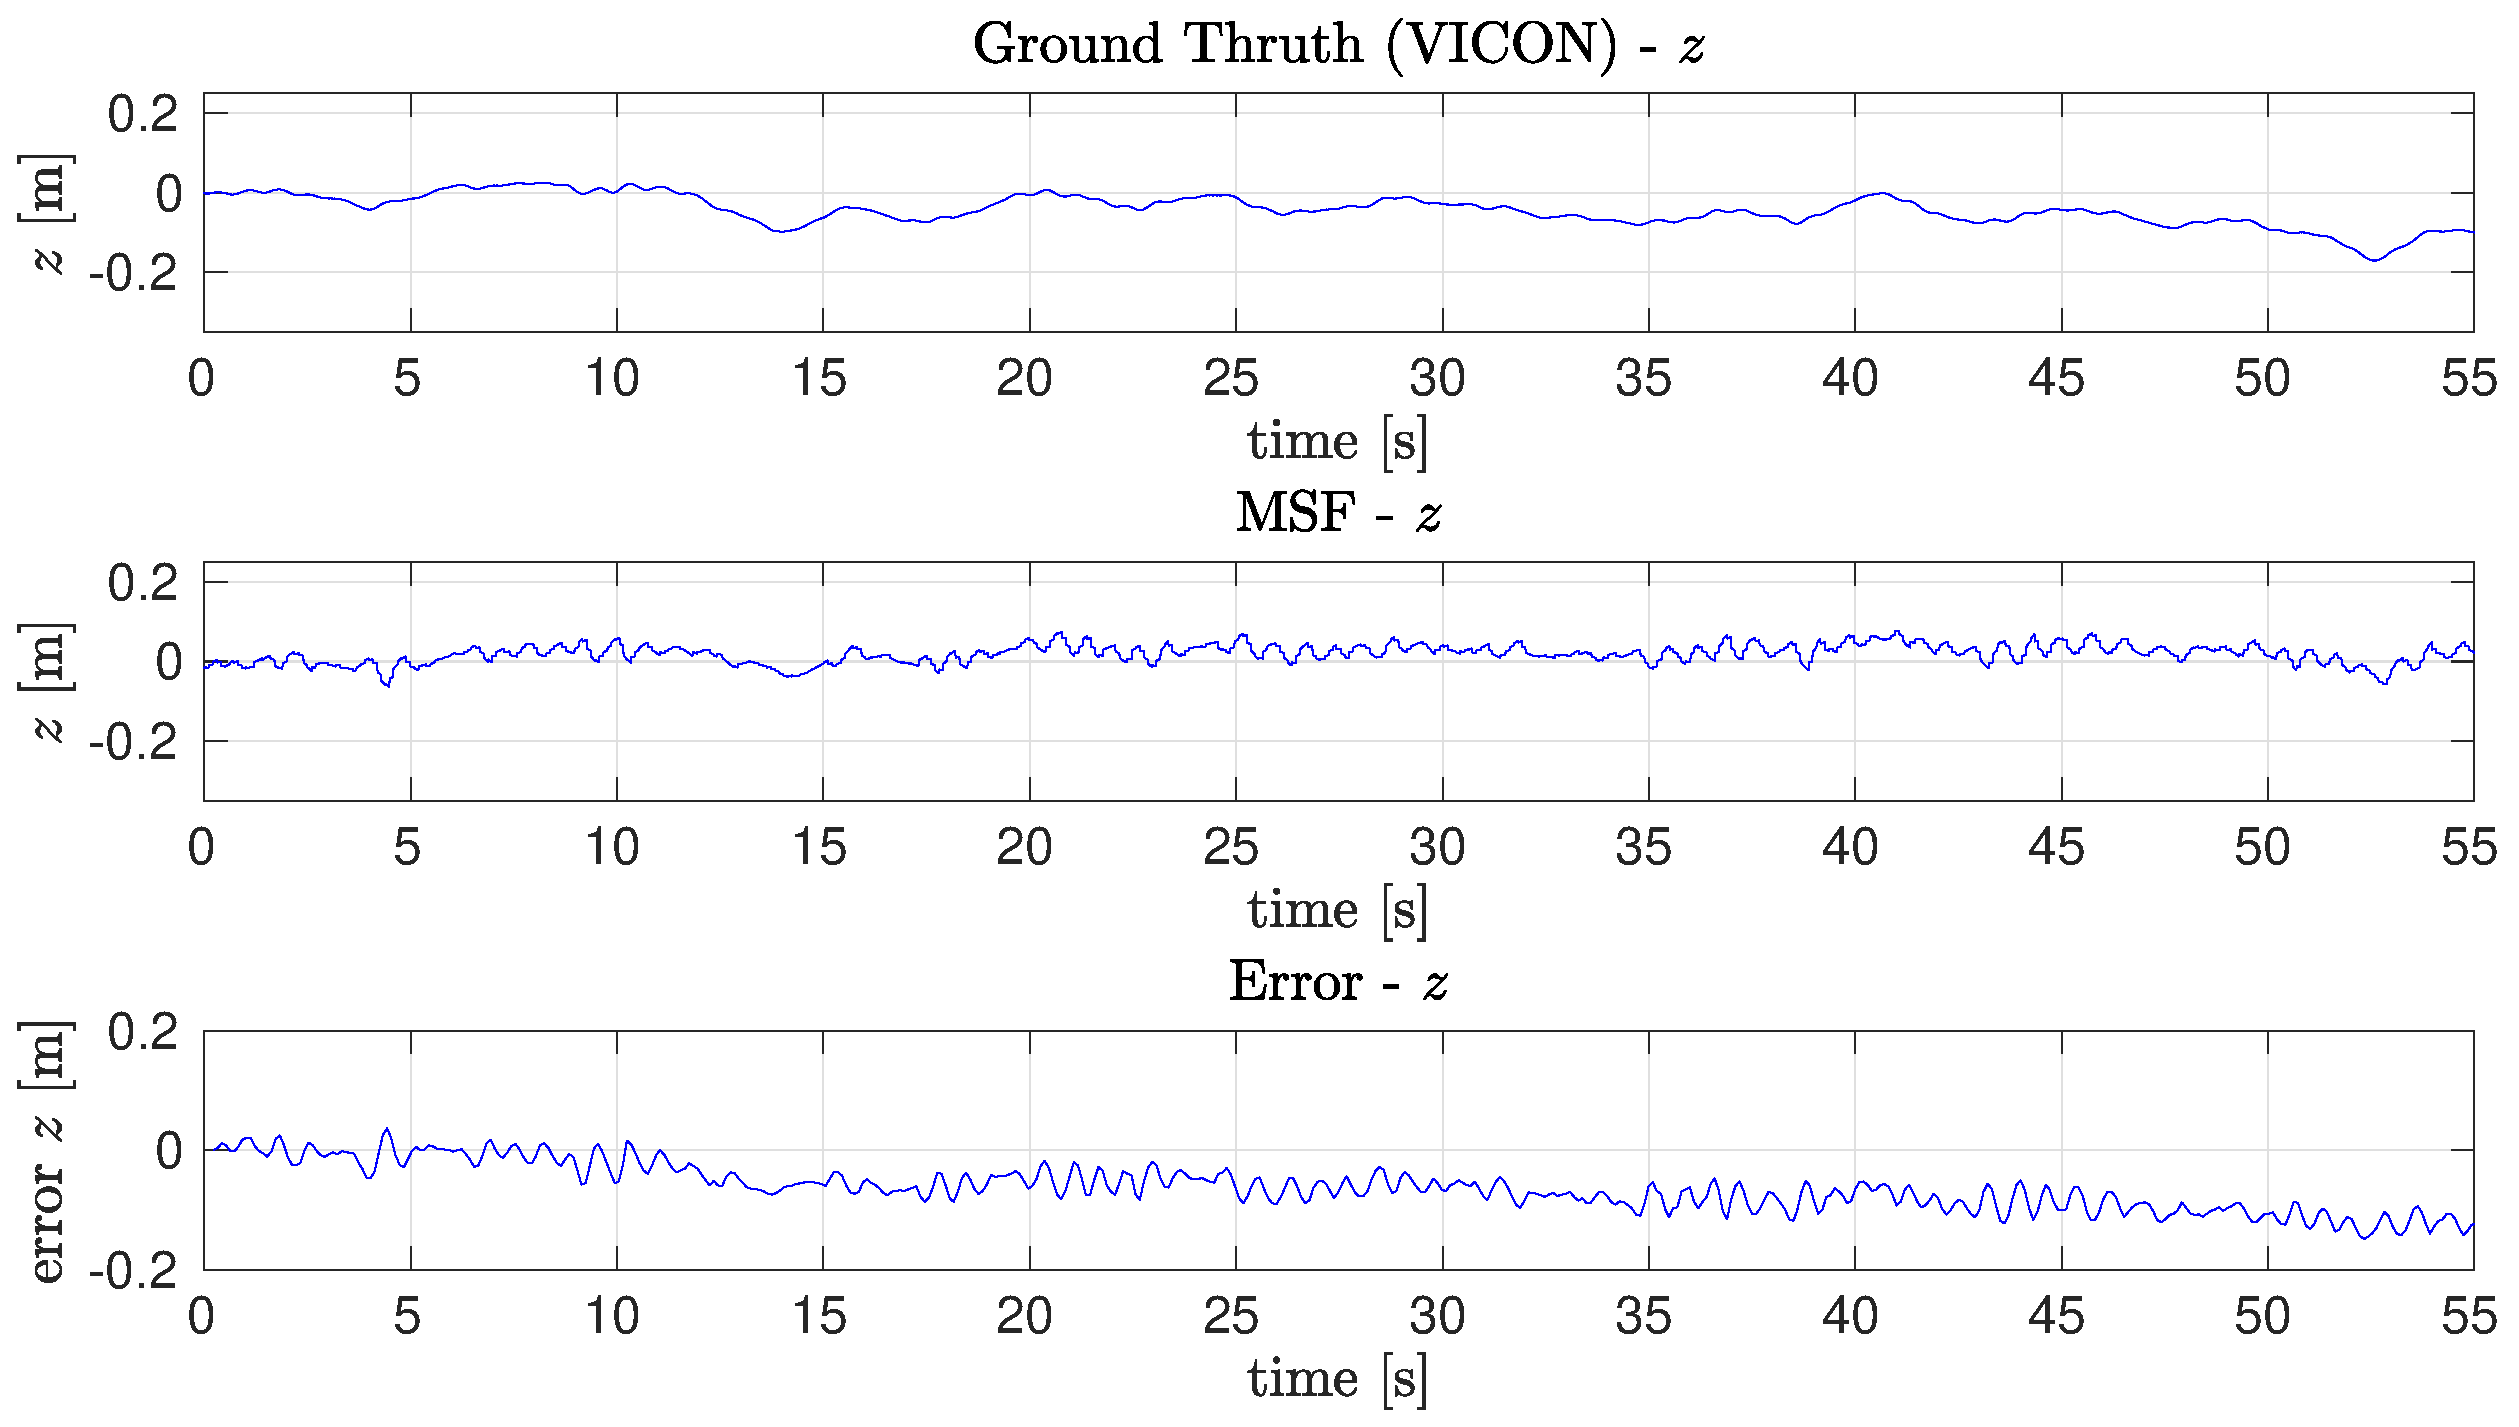
\includegraphics[width=1\textwidth]{images/res_z}
\caption{Relative pose estimation, while the \ac{UAV} is hovering, in the $z$ 
axis of the \ac{MSF} filter and the Vicon ground truth, and the difference 
between them.}
\label{fig:res_z}
\end{figure}



